\documentclass[11pt]{article}
% Shared preamble of the project's LaTeX notes: notes/*.tex and the documents in literature/.
% Project macros go at the end. A macro copied from a paper's source goes in the note that
% quotes it, between its \input of this file and \begin{document}.
\usepackage[a4paper,margin=25mm]{geometry}
\usepackage{amsmath,amssymb,mathtools,bm}
\usepackage{graphicx,booktabs,xltabular}
\usepackage{xcolor}
\usepackage{xspace}
\usepackage[numbers,sort&compress]{natbib}
\bibliographystyle{apsrev4-2} % prints the arXiv ID of each entry in refs.bib
\usepackage[colorlinks,allcolors=blue!60!black]{hyperref}
\usepackage[notref,notcite]{showkeys} % prints each \label in the margin, so a pointer by label is found in the PDF
\renewcommand*\showkeyslabelformat[1]{\normalfont\tiny\ttfamily#1}

% Ragged-right X column for tables with prose cells: bridges, the survey's term map.
\newcolumntype{L}{>{\raggedright\arraybackslash}X}

% Project macros, in the notation of CONVENTIONS.md.
\newcommand{\GeV}{\mathrm{GeV}}
\newcommand{\MeV}{\mathrm{MeV}}
\newcommand{\vep}{{\bm p}}
\newcommand{\vek}{{\bm k}}
\newcommand{\veq}{{\bm q}}
\newcommand{\ver}{{\bm r}}
\newcommand{\vex}{{\bm x}}
\newcommand{\veA}{{\bm A}}
\newcommand{\vetau}{{\bm \tau}}
\newcommand{\veL}{{\bm L}}
\newcommand{\veS}{{\bm S}}
\newcommand{\ven}{{\bm n}}
\newcommand{\veep}{{\bm \epsilon}}
\newcommand{\veepst}{{\bm \epsilon}^{\prime*}}
\newcommand{\bbnP}{[\bar{b}b]_1(nP)}
\newcommand{\bbarb}{[\bar{b}b]_1}
\newcommand{\psibb}{\Psi^{(\bar{b}b)}}
\newcommand{\Mbb}{M^{(\bar{b}b)}}
\newcommand{\X}{X(3872)}
\newcommand{\Xb}{X_b}
\newcommand{\VQQ}{V^{(\bar{b}b)}}
\newcommand{\VOME}{V^{\rm (OME)}}
\newcommand{\TOME}{T^{\rm (OME)}}
\newcommand{\BOchiEFT}{BO$\chi$EFT\xspace}
\newcommand{\cyan}[1]{\textcolor{cyan}{#1}}

\title{title=continuation}
\newcommand{\todo}{\textcolor{red}{TO BE ADDED}}
\newcommand{\VS}{V_{\Sigma_g^+}}
\newcommand{\VP}{V_{\Pi_g}}
% ---------------------------------------------------------------- added: the change markup and tags of main.tex
\usepackage{braket}
\usepackage{tikz}
\usepackage[most]{tcolorbox}
\usepackage[normalem]{ulem}
\setlength{\emergencystretch}{2em} % struck-out text (\sout) cannot hyphenate
\newcommand{\Pbb}{{\cal P}_{\bar bb}}
\newcommand{\tagP}[1]{\textcolor{blue!65!black}{\textsf{\small[P:\,#1]}}}
\newcommand{\tagD}{\textcolor{orange!85!black}{\textsf{\small[D]}}}
% \showaitrue : additions in magenta with a left bar; replaced text struck through in gray.
% \showaifalse: clean text (additions printed plain, struck text dropped).
\newif\ifshowai
\showaitrue
\colorlet{aicolor}{magenta!75!black}
\ifshowai
	\newcommand{\ai}[1]{\textcolor{aicolor}{#1}}
	\newcommand{\aifix}[2]{\textcolor{gray}{\sout{#1}} \textcolor{aicolor}{#2}}
	\newcommand{\aifixm}[2]{\textcolor{gray}{\text{\sout{$#1$}}}\,\textcolor{aicolor}{#2}}
	\newtcolorbox{aiadd}{blanker,breakable,parbox=false,coltext=aicolor,borderline west={1.5pt}{-6pt}{aicolor},
		before skip=0.5em,after skip=0.5em}
\else
	\newcommand{\ai}[1]{#1}
	\newcommand{\aifix}[2]{#2}
	\newcommand{\aifixm}[2]{#2}
	\newenvironment{aiadd}{\par}{\par}
\fi
\author{}
\date{2026-11-05}
\begin{document}
\maketitle

\aifix{this is about s-channel exchange of bottomonium states, next}{That was the $s$-channel exchange of bottomonium states. Next} we are going to see the short range counterterm and why it's a constant at LO.

with the transformation defined above, we can transform the potential from BO basis to partial wave basis \ai{(the matrix $U$ at the end of the first part, $\ket{\rm BO}=U\ket{\rm PW}$ \tagP{Eq.~(22)})}

\begin{equation}
	V(r) = U^T \text{diag}(\aifixm{V_{\Sigma_g^+}}{V_{\Sigma_g^{+\prime}}}, V_{\Pi_g}, V_{\Pi_g})U
\end{equation}
\ai{Why $U^T\cdots U$: $\hat V=\sum_i\ket{{\rm BO}_i}V_i\bra{{\rm BO}_i}$ and $\braket{\alpha|{\rm BO}_i}=U_{i\alpha}$, so $V_{\alpha\beta}=\sum_iU_{i\alpha}V_iU_{i\beta}$ \tagP{Eq.~(24)}. And the level is $\Sigma_g^{+\prime}$, the meson-pair configuration, not the string $\Sigma_g^+$ of the compact state (the same correction as in the first part).}

And note that the diagonal potential in BO basis can be separated into two \aifix{part}{parts}

\begin{equation}
	\text{diag}(\aifixm{V_{\Sigma_g^+}}{V_{\Sigma_g^{+\prime}}}, V_{\Pi_g}, V_{\Pi_g}) = V_{\Pi_g} {\bm 1} + (\aifixm{V_{\Sigma_g^+}}{V_{\Sigma_g^{+\prime}}} - V_{\Pi_g}) \text{diag}(1,0,0)
\end{equation}

then we have the potential in partial wave channel reads \aifix{\todo}{}

\begin{aiadd}
	First what it means. In the static limit $m_b\to\infty$ the $b$ and $\bar b$ sit still at distance $r$: no heavy kinetic energy, no $B^*$--$B$ splitting, no OME recoil \tagP{l.\,541}. At each $r$ the light degrees of freedom then have energy levels, and these are the BO potentials. The two $\Pi_g$ configurations ($J_l=1,2$) share one potential $V_{\Pi_g}(r)$. So the decomposition above says: every channel is shifted by the common $V_{\Pi_g}$, and only the difference $V_{\Sigma_g^{+\prime}}-V_{\Pi_g}$ knows about the special direction $\Sigma_g^{+\prime}$.

	Now multiply out. The unit matrix goes through, $U^T\bm 1U=\bm 1$. For the rest write $\text{diag}(1,0,0)=e_1e_1^T$ with $e_1=(1,0,0)^T$. Then $U^Te_1$ is the first row of $U$ written as a column, i.e.\ the vector of overlaps $u_\alpha=\braket{\alpha|\Sigma_g^{+\prime}}$. So
	\[
		u=U^Te_1=\begin{pmatrix}1/\sqrt3\\ 1/\sqrt6\\ -1/\sqrt2\end{pmatrix},\qquad
		V(r)=V_{\Pi_g}(r)\,\bm 1+\big[V_{\Sigma_g^{+\prime}}(r)-V_{\Pi_g}(r)\big]\,uu^T .
	\]
	This is \tagP{Eq.~(25)}. The rank-one matrix is
	\[
		uu^T=\begin{pmatrix}
			\frac13           & \frac{1}{3\sqrt2}  & -\frac{1}{\sqrt6}  \\[1mm]
			\frac{1}{3\sqrt2} & \frac16            & -\frac{1}{2\sqrt3} \\[1mm]
			-\frac{1}{\sqrt6} & -\frac{1}{2\sqrt3} & \frac12
		\end{pmatrix}
		=\frac13\bm 1-\frac16\begin{pmatrix}0&-\sqrt2&\sqrt6\\ -\sqrt2&1&\sqrt3\\ \sqrt6&\sqrt3&-1\end{pmatrix},
	\]
	where we pulled out the trace part, $\text{tr}\,uu^T=u^Tu=1$ (check two entries: $-\frac16\cdot(-\sqrt2)=\frac{1}{3\sqrt2}$ and $\frac13-\frac16=\frac16$). Collecting the unit matrices,
	\[
		V(r)=V_C(r)\,\bm 1+V_T(r)\begin{pmatrix}0&-\sqrt2&\sqrt6\\ -\sqrt2&1&\sqrt3\\ \sqrt6&\sqrt3&-1\end{pmatrix},\qquad
		V_C=\frac{V_{\Sigma_g^{+\prime}}+2V_{\Pi_g}}{3},\quad V_T=\frac{V_{\Pi_g}-V_{\Sigma_g^{+\prime}}}{6},
	\]
	which is \tagP{Eqs.~(26)--(27)}. $V_C$ is the same in all channels, like a central force; the matrix multiplying $V_T$ is traceless and couples $S$ to $D$, like the tensor force of OPE. Hence the names.

	Two remarks. (i) $V(r)$ is only the potential. In the radial Schr\"odinger equation the centrifugal barrier $L_\alpha(L_\alpha+1)/(2\mu_\alpha r^2)$ and the threshold $\Delta m$ of channel 3 come on top of it \tagP{Eq.~(28)}; they are kinematics, not part of $V_C$ or $V_T$. (ii) $V(r)$ is static and local, and we do not use it as our interaction: its long-range part is our OME and its short-range part our contact terms. That is what the next question is about.
\end{aiadd}

actually I'm not super sure what's this part of the paper doing, Matching BO to partial-wave potentials, why computing $C_{T,n}^<$, what is this trying to say, please finish this for me

\begin{aiadd}
	\textbf{Answer.} The section asks what the BO picture says about the \emph{short-range} part of the meson--meson interaction. It does not add a new potential.

	\textbf{What is matched.} $V_{\Sigma_g^{+\prime}}(r)$ and $V_{\Pi_g}(r)$ are energies of the whole light cloud. At large $r$ the two mesons are far apart and exchange pions and etas; that part is our OME \tagP{l.\,618--620}. At short $r$ the mesons overlap and the light quarks rearrange. Our hadronic theory cannot resolve this, so it is replaced by contact terms, $\delta^{(3)}(\vec r)$ and its derivatives \tagP{l.\,621--626}. The questions are: which contact term comes first, and what does the cylindrical symmetry say about the others?

	\textbf{Step 1: momentum space.} We need the partial-wave states \tagP{Eqs.~(30)--(31)}
	\[
		\braket{p',\alpha'|p,\alpha}=\delta_{\alpha'\alpha}\frac{2\pi^2}{p^2}\delta(p'-p),\qquad
		\braket{\vec r|p,\alpha}=4\pi\,i^{L_\alpha}j_{L_\alpha}(pr)\,\mathcal Y_\alpha(\hat r),\qquad
		\int d\Omega\,\mathcal Y_{\alpha'}^\dagger\mathcal Y_\alpha=\frac{\delta_{\alpha'\alpha}}{4\pi}.
	\]
	(The two are consistent: with $\int_0^\infty r^2dr\,j_L(p'r)j_L(pr)=\frac{\pi}{2p^2}\delta(p'-p)$ one gets $(4\pi)^2\cdot\frac{1}{4\pi}\cdot\frac{\pi}{2p^2}=\frac{2\pi^2}{p^2}$.) Insert $\int d^3r\,\ket{\vec r}\bra{\vec r}$ on both sides of a local $\hat V$:
	\begin{align*}
		V_{\alpha'\alpha}(p',p) & =(4\pi)^2(-i)^{L_{\alpha'}}i^{L_\alpha}\int_0^\infty r^2dr\,j_{L_{\alpha'}}(p'r)\,j_{L_\alpha}(pr)\int d\Omega\,\mathcal Y_{\alpha'}^\dagger\hat V\mathcal Y_\alpha \\
		                        & =4\pi\,i^{L_\alpha-L_{\alpha'}}\int_0^\infty r^2dr\,j_{L_{\alpha'}}(p'r)\,V_{\alpha'\alpha}(r)\,j_{L_\alpha}(pr),
	\end{align*}
	with $V_{\alpha'\alpha}(r)=4\pi\int d\Omega\,\mathcal Y_{\alpha'}^\dagger\hat V\mathcal Y_\alpha$ the matrix above \tagP{Eq.~(32)}. The phase $i^{L_\alpha-L_{\alpha'}}$ is $+1$ for $S$--$S$ and $D$--$D$, and $-1$ for $S$--$D$.

	\textbf{Step 2: short range means small argument.} If a piece of the interaction only lives at $r\lesssim R=1/\Lambda_\chi$ and $p,p'\ll\Lambda_\chi$, expand the Bessel functions \tagP{Eq.~(33)}:
	\[
		j_L(x)=\frac{x^L}{(2L+1)!!}\Big(1-\frac{x^2}{2(2L+3)}+\dots\Big),\qquad
		j_0(x)=1-\frac{x^2}{6}+\dots,\qquad
		j_2(x)=\frac{x^2}{15}-\frac{x^4}{210}+\dots
	\]
	So the leading term of a short-range piece is
	\[
		V^<_{\alpha'\alpha}(p',p)\simeq4\pi\,i^{L_\alpha-L_{\alpha'}}\,\frac{p'^{L_{\alpha'}}p^{L_\alpha}}{(2L_{\alpha'}+1)!!\,(2L_\alpha+1)!!}\int_0^Rdr\,r^{2+L_{\alpha'}+L_\alpha}\,V_{\alpha'\alpha}(r):
	\]
	$S$--$S$ starts with a constant, $S$--$D$ with $p^2$ (or $p'^2$), $D$--$D$ with $p'^2p^2$.

	\textbf{Step 3: so the LO contact is a constant, in channel 1 only.} Counting $p,p'\sim Q$, only the $S$--$S$ term is $\mathcal O(Q^0)$, and the only $S$ wave in $1^{++}$ is channel 1:
	\[
		V^{\rm CT}_{\alpha'\alpha}(p',p)=C\,\delta_{\alpha'1}\delta_{\alpha1}+\mathcal O(Q^2).
	\]
	In $r$ space this is $C\,\delta^{(3)}(\vec r)$ \tagP{l.\,634}. That is all we need for the LO statement.

	\textbf{Step 4: what $C^<_{T,n}$ is for.} The paper then asks how large the \emph{higher} $S$--$D$ and $D$--$D$ contact terms are, using what is known about the static levels at short distance. Both levels come from the same light-quark multiplet as $r\to0$, so their difference starts at $r^2$ \tagP{Eq.~(34)}:
	\[
		V_T(r)=b_Tr^2+c_Tr^4+\dots,\qquad b_T=\tfrac16(b_\Pi-b_\Sigma),\quad c_T=\tfrac16(c_\Pi-c_\Sigma).
	\]
	Put the tensor entries $V_{12}=-\sqrt2V_T$, $V_{13}=\sqrt6V_T$, $V_{23}=\sqrt3V_T$ into Step 1 and cut the integral at $R=1/\Lambda_\chi$. After expanding the Bessel functions only radial moments of $V_T$ appear, and the paper gives them a name \tagP{Eq.~(35)}:
	\[
		C^<_{T,n}\equiv4\pi\int_0^{1/\Lambda_\chi}dr\,r^nV_T(r)=4\pi\Big[\frac{b_T}{(n+3)\Lambda_\chi^{n+3}}+\frac{c_T}{(n+5)\Lambda_\chi^{n+5}}\Big].
	\]
	For $V^<_{12}$ (outgoing $S$, incoming $D$, phase $i^2=-1$):
	\begin{align*}
		j_0(p'r)j_2(pr) & =\Big(1-\frac{p'^2r^2}{6}\Big)\Big(\frac{p^2r^2}{15}-\frac{p^4r^4}{210}\Big)+\dots                 \\
		                & =\frac{p^2}{15}\,r^2-\Big(\frac{p'^2p^2}{90}+\frac{p^4}{210}\Big)r^4+\dots,                        \\
		V^<_{12}        & =4\pi\,(-1)(-\sqrt2)\int_0^Rdr\,r^2\,j_0(p'r)j_2(pr)\,V_T(r)                                       \\
		                & =\frac{\sqrt2}{15}\Big[p^2C^<_{T,4}-\Big(\frac{p'^2p^2}{6}+\frac{p^4}{14}\Big)C^<_{T,6}\Big]+\dots
	\end{align*}
	$V^<_{13}$ has the same $L$'s and phase but $\sqrt6$ instead of $-\sqrt2$, so $V^<_{13}=-\sqrt3\,V^<_{12}$: a relation from HQSS, through the static channel matrix. For $V^<_{23}$ ($D$--$D$, phase $+1$), $j_2(p'r)j_2(pr)=\frac{p'^2p^2r^4}{225}+\dots$ gives $V^<_{23}=\frac{\sqrt3}{225}\,p'^2p^2\,C^<_{T,6}+\dots$. The reversed entries follow from $V^<_{ji}(p',p)=V^<_{ij}(p,p')$ \tagP{Eq.~(36)}.

	\textbf{Step 5: two separate suppressions.} The momentum powers $p'^{L'}p^L$ of Step 2 come from angular momentum alone. Step 4 adds a second one: $b_T$ and $c_T$ are nonperturbative, naturally $\sim\Lambda_{\rm QCD}^3$ and $\Lambda_{\rm QCD}^5$, so each further term of the multipole expansion costs $(\Lambda_{\rm QCD}/\Lambda_\chi)^2$ (compare the two terms of $C^<_{T,n}$). The paper counts this factor as $\mathcal O(Q^2)$ and says the assignment can be adjusted \tagP{l.\,668}. With it, higher BO terms enter channel 1 at $\mathcal O(Q^2)$, and the $D$-wave and off-diagonal entries at $\mathcal O(Q^4)$ or later \tagP{l.\,669}. Step 3 does not need this extra counting.

	\textbf{What it does not do.} It does not give a value of $C$. The moments depend on the arbitrary radius $1/\Lambda_\chi$, OME has its own short-range piece whose split from the contacts is scheme dependent, and $C$ must still be fitted at each cutoff \tagP{l.\,626, 670}. And the static $V(r)$ is not added on top of OME and $C$: the potential we use stays full OME $+\,\VQQ+C$.
\end{aiadd}

\aifix{\todo: add the definitions of fields}{}

\begin{aiadd}
	The heavy mesons are collected in $2\times2$ matrices in spin space \tagP{Eq.~(64)}:
	\[
		H_a=P_a+\bm V_a\cdot\bm\sigma,\qquad \bar H_a=\bar P_a+\bar{\bm V}_a\cdot\bm\sigma .
	\]
	\begin{itemize}
		\item $P_a=(B^-,\bar B^0)$ and $V^i_a=(B^{*-},\bar B^{*0})$ annihilate the $b\bar q$ mesons; $\bar P_a=(B^+,B^0)$ and $\bar V^i_a=(B^{*+},B^{*0})$ annihilate the $\bar bq$ mesons. The bar means antimeson, not complex conjugation.
		\item $a=1,2$ is the light flavour ($u,d$) and $i=1,2,3$ the vector index of the $B^*$. The $\bm\sigma$ act on spin; the flavour Pauli matrices are called $\tau_a$. Spin and flavour are two different $2\times2$ spaces.
		\item The traces in $\mathcal L_\Phi$ are over spin; the flavour indices are written out.
		\item Charge conjugation: $\mathcal CP_a\mathcal C^{-1}=\bar P_a$, $\mathcal CV^i_a\mathcal C^{-1}=-\bar V^i_a$, so the $C$-even state is $\ket{B\bar B^*;C{=}+}=\big(\ket{B\bar B^*}-\ket{B^*\bar B}\big)/\sqrt2$, with a minus \tagP{l.\,952 and its footnote}.
		\item The pseudo-Goldstone bosons sit in the flavour matrix $\Phi$ below and enter through the axial field $\bm u=-\nabla\Phi/F_\pi+\mathcal O(\Phi^3)$, with $F_\pi=92.2\,\MeV$ \tagP{l.\,984}.
	\end{itemize}
	We take this Lagrangian as given (it is the LO term of heavy-meson chiral perturbation theory) and don't rederive it from symmetry.
\end{aiadd}

As for the t-channel meson exchanges, OME potential is built from the LO chiral Lagrangian \aifix{describring}{describing} heavy-light mesons with the pseudo-Nambu-Goldstone bosons.

\[
	\mathcal{L}_{\Phi} = -\frac{g_b}{4}\mathrm{Tr}\left(H_a^\dagger H_b \bm{\sigma}\cdot \bm{u}_{ba}\right) + \frac{g_b}{4}\mathrm{Tr}\left(\bm{\sigma}\cdot\bm{u}_{ab}\aifixm{\hat H_b \hat H_a^\dagger}{\bar H_b\bar H_a^\dagger}\right)
\]
\ai{\tagP{Eq.~(65)}; the antimeson field is $\bar H$.} \aifix{bottom-meson}{The bottom-meson} axial coupling is determined at physical bottom-quark mass using lattice-QCD techniques\ai{: $g_b=0.56(3)_{\rm stat}(7)_{\rm sys}$, and we use the central value \tagP{Eq.~(66)}}.

the matrix of pseudoscalar fields
\[
	\Phi = \pi_a\tau_a + \frac{\eta}{\sqrt{3}}\aifixm{1}{\bm 1} = \begin{pmatrix}
		\aifixm{\pi^0}{\pi^0+\frac{1}{\sqrt3}\eta} & \aifixm{\frac{1}{\sqrt{3}}\eta}{\sqrt2\pi^+}          \\
		\sqrt{2}\pi^-                              & -\pi^0+\aifixm{\frac{1}{3}\eta}{\frac{1}{\sqrt3}\eta}
	\end{pmatrix}
\]
\ai{with $\pi^\pm=(\pi_1\mp i\pi_2)/\sqrt2$ \tagP{Eq.~(67)}. Check: $\pi_a\tau_a$ has $\pm\pi_3$ on the diagonal and $\pi_1\mp i\pi_2=\sqrt2\pi^\pm$ off the diagonal, upper right and lower left; and $\eta$ multiplies the unit matrix, so it sits on \emph{both} diagonal entries with the same $1/\sqrt3$.}

The LO \aifix{lagrangian of}{Lagrangian coupling} a single $\Phi$ field to \ai{a} pair of heavy-light mesons takes \ai{the} form \aifix{\todo}{}

\begin{aiadd}
	Insert $u^k_{ab}=-\partial_k\Phi_{ab}/F_\pi$ and do the spin traces with
	$\mathrm{Tr}\,\sigma_i=0$, $\mathrm{Tr}\,\sigma_i\sigma_j=2\delta_{ij}$, $\mathrm{Tr}\,\sigma_i\sigma_j\sigma_k=2i\varepsilon_{ijk}$.

	\textbf{Meson term.}
	\begin{align*}
		H_a^\dagger H_b                                & =P_a^\dagger P_b+P_a^\dagger V_b^j\sigma_j+V_a^{i\dagger}P_b\sigma_i+V_a^{i\dagger}V_b^j\sigma_i\sigma_j, \\
		\mathrm{Tr}\big(H_a^\dagger H_b\,\sigma_k\big) & =2\big(P_a^\dagger V_b^k+V_a^{k\dagger}P_b\big)+2i\varepsilon_{ijk}V_a^{i\dagger}V_b^j .
	\end{align*}
	The $P^\dagger P$ term drops ($\mathrm{Tr}\,\sigma_k=0$): there is no $BB\phi$ vertex, since $0^-\to0^-0^-$ is forbidden by parity and angular momentum together. So
	\[
		-\frac{g_b}{4}\mathrm{Tr}\big(H_a^\dagger H_b\,\sigma_ku^k_{ba}\big)
		=\frac{g_b}{2F_\pi}\Big[\big(V_a^{k\dagger}P_b+P_a^\dagger V_b^k\big)\partial_k\Phi_{ba}+i\varepsilon_{ijk}V_a^{i\dagger}V_b^j\,\partial_k\Phi_{ba}\Big].
	\]
	\textbf{Antimeson term.} Now the order is $\sigma_k\bar H_b\bar H_a^\dagger$, so the three Pauli matrices come in the opposite order, $\mathrm{Tr}\,\sigma_k\sigma_j\sigma_i=-2i\varepsilon_{ijk}$, and after normal ordering the boson fields
	\[
		\mathrm{Tr}\big(\sigma_k\bar H_b\bar H_a^\dagger\big)=2\big(\bar P_a^\dagger\bar V_b^k+\bar V_a^{k\dagger}\bar P_b\big)-2i\varepsilon_{ijk}\bar V_a^{i\dagger}\bar V_b^j .
	\]
	With the $+$ sign in front of this term,
	\[
		\frac{g_b}{4}\mathrm{Tr}\big(\sigma_ku^k_{ab}\bar H_b\bar H_a^\dagger\big)
		=\frac{g_b}{2F_\pi}\Big[-\big(\bar P_a^\dagger\bar V_b^k+\bar V_a^{k\dagger}\bar P_b\big)\partial_k\Phi_{ab}+i\varepsilon_{ijk}\bar V_a^{i\dagger}\bar V_b^j\,\partial_k\Phi_{ab}\Big].
	\]
	Together this is the paper's one-boson Lagrangian \tagP{Eq.~(68)}. Note the pattern: for antimesons the $PV\phi$ term flips sign and the $VV\phi$ term does not; and the flavour indices appear as $\Phi_{ba}$ for mesons but $\Phi_{ab}$ for antimesons.
\end{aiadd}

\aifix{\todo: add the vertices from the paper}{}

\begin{aiadd}
	Take a meson line with incoming momentum $\bm p$ and outgoing $\bm p'$; it loses $\bm q=\bm p-\bm p'$. The gradient on the emitted or absorbed boson gives a common factor $\pm i\bm q$; stripping it and the flavour matrix, Eq.~(68) gives two vertices \tagP{Eqs.~(69)--(70)}
	\[
		v^a_{B^*B\phi}=\frac{g_b}{2F_\pi}\,\tau^a\,(\bm\epsilon\cdot\bm q),\qquad
		v^a_{B^*B^*\phi}=-\frac{g_b}{\sqrt2F_\pi}\,\tau^a\,(\bm A\cdot\bm q),\qquad
		\bm A=\frac{i}{\sqrt2}\,\bm\epsilon\times\bm\epsilon'^*,
	\]
	with $\bm\epsilon=\bm\epsilon_\lambda(\bm p)$ the incoming and $\bm\epsilon'^*=\bm\epsilon^*_{\lambda'}(\bm p')$ the outgoing polarisation. For $\eta$ exchange replace $\tau^a$ by $\bm 1/\sqrt3$.
	\begin{itemize}
		\item $PV\phi$: the field $V^k$ (or $V^{k\dagger}$) becomes the polarisation of the one vector meson, so the vertex is $\bm\epsilon\cdot\bm q$ (or $\bm\epsilon'^*\cdot\bm q$ for an outgoing $B^*$).
		\item $VV\phi$: $i\varepsilon_{ijk}\epsilon'^*_i\epsilon_jq_k=i(\bm\epsilon'^*\times\bm\epsilon)\cdot\bm q=-i(\bm\epsilon\times\bm\epsilon'^*)\cdot\bm q=-\sqrt2\,\bm A\cdot\bm q$. With the prefactor $\frac{g_b}{2F_\pi}$ this is the $-\frac{g_b}{\sqrt2F_\pi}$ above.
		\item Antimesons: in the c.m.\ frame the antimeson goes from $-\bm p$ to $-\bm p'$, so it loses $-\bm q$. Its $PV\phi$ vertex has the extra minus of Eq.~(68), its $VV\phi$ vertex does not.
	\end{itemize}
	For the signs of whole diagrams we need the Hamiltonian matrix elements with the $i$'s. With $H_{\rm int}=-\int d^3x\,\mathcal L_\Phi$ and $c\equiv g_b/(2F_\pi)$, emitting a boson of momentum $\bm k$ gives $\nabla\to-i\bm k$ and absorbing it $\nabla\to+i\bm k$. Per unit flavour factor (and $1/\sqrt{2E_\phi}$):
	\begin{center}
		\begin{tabular}{lcc}
			                                & emit $\phi(\bm k)$              & absorb $\phi(\bm k)$            \\ \hline
			meson $B\to B^*$                & $+ic\,\bm\epsilon'^*\cdot\bm k$ & $-ic\,\bm\epsilon'^*\cdot\bm k$ \\
			antimeson $\bar B^*\to\bar B$   & $-ic\,\bm\epsilon\cdot\bm k$    & $+ic\,\bm\epsilon\cdot\bm k$    \\
			meson or antimeson $B^*\to B^*$ & $-i\sqrt2c\,\bm A\cdot\bm k$    & $+i\sqrt2c\,\bm A\cdot\bm k$
		\end{tabular}
	\end{center}
	The meson $B^*\to B$ and antimeson $\bar B\to\bar B^*$ entries are the same with $\bm\epsilon'^*$ and $\bm\epsilon$ interchanged.
\end{aiadd}

There are four intermediate states in total \aifix{\todo: add the TOPT diagrams}{}

\begin{aiadd}
	\textbf{What TOPT does.} OME is second order in $H_{\rm int}$. In time-ordered (old-fashioned) perturbation theory every particle stays on its mass shell; energy is conserved overall but not at each vertex, and the price is an energy denominator for the intermediate state:
	\[
		V=\sum_n\frac{\braket{f|H_{\rm int}|n}\braket{n|H_{\rm int}|i}}{M-E_n+i0}.
	\]
	Between the two vertices there are three particles, the two heavy mesons and $\phi$, and which ones depends on who emits first. The four classes are \tagP{Eq.~(71)}
	\[
		\beta=1:\ B\bar B\phi,\qquad \beta=2:\ B^*\bar B^*\phi,\qquad \beta=3:\ B\bar B^*\phi,\qquad \beta=4:\ \bar B^*B\phi .
	\]
	The diagrams show them for $B\bar B^*\to B^*\bar B$ ($\beta=1,2$), $B\bar B^*\to B^*\bar B^*$ ($\beta=3$) and $B^*\bar B^*\to B\bar B^*$ ($\beta=4$). Time runs to the right, single lines are $B$, double lines $B^*$, and the thin vertical line cuts the intermediate state.
	\begin{center}
		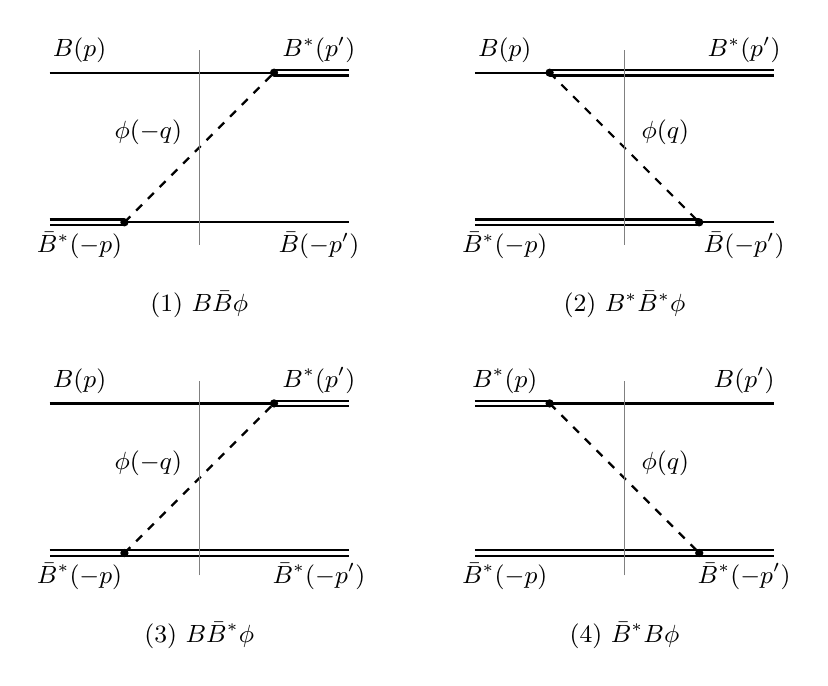
\begin{tikzpicture}[black,x=0.95cm,y=0.95cm,font=\small,
				Bl/.style={thick},Bs/.style={thick,double,double distance=1.2pt},
				ph/.style={thick,dashed},cut/.style={gray}]
			% (1): the antimeson emits first
			\begin{scope}
				\draw[Bl] (0,2)--(3,2); \draw[Bs] (3,2)--(4,2);
				\draw[Bs] (0,0)--(1,0); \draw[Bl] (1,0)--(4,0);
				\draw[ph] (1,0)--(3,2); \draw[cut] (2,-0.3)--(2,2.3);
				\fill (1,0) circle (1.5pt); \fill (3,2) circle (1.5pt);
				\node[above] at (0.4,2) {$B(\bm p)$}; \node[above] at (3.6,2) {$B^*(\bm p')$};
				\node[below] at (0.4,0) {$\bar B^*(-\bm p)$}; \node[below] at (3.6,0) {$\bar B(-\bm p')$};
				\node[left] at (1.9,1.2) {$\phi(-\bm q)$};
				\node at (2,-1.1) {(1) $B\bar B\phi$};
			\end{scope}
			% (2): the meson emits first
			\begin{scope}[xshift=5.4cm]
				\draw[Bl] (0,2)--(1,2); \draw[Bs] (1,2)--(4,2);
				\draw[Bs] (0,0)--(3,0); \draw[Bl] (3,0)--(4,0);
				\draw[ph] (1,2)--(3,0); \draw[cut] (2,-0.3)--(2,2.3);
				\fill (1,2) circle (1.5pt); \fill (3,0) circle (1.5pt);
				\node[above] at (0.4,2) {$B(\bm p)$}; \node[above] at (3.6,2) {$B^*(\bm p')$};
				\node[below] at (0.4,0) {$\bar B^*(-\bm p)$}; \node[below] at (3.6,0) {$\bar B(-\bm p')$};
				\node[right] at (2.1,1.2) {$\phi(\bm q)$};
				\node at (2,-1.1) {(2) $B^*\bar B^*\phi$};
			\end{scope}
			% (3): the antimeson emits first
			\begin{scope}[yshift=-4.2cm]
				\draw[Bl] (0,2)--(3,2); \draw[Bs] (3,2)--(4,2);
				\draw[Bs] (0,0)--(4,0);
				\draw[ph] (1,0)--(3,2); \draw[cut] (2,-0.3)--(2,2.3);
				\fill (1,0) circle (1.5pt); \fill (3,2) circle (1.5pt);
				\node[above] at (0.4,2) {$B(\bm p)$}; \node[above] at (3.6,2) {$B^*(\bm p')$};
				\node[below] at (0.4,0) {$\bar B^*(-\bm p)$}; \node[below] at (3.6,0) {$\bar B^*(-\bm p')$};
				\node[left] at (1.9,1.2) {$\phi(-\bm q)$};
				\node at (2,-1.1) {(3) $B\bar B^*\phi$};
			\end{scope}
			% (4): the meson emits first
			\begin{scope}[xshift=5.4cm,yshift=-4.2cm]
				\draw[Bs] (0,2)--(1,2); \draw[Bl] (1,2)--(4,2);
				\draw[Bs] (0,0)--(4,0);
				\draw[ph] (1,2)--(3,0); \draw[cut] (2,-0.3)--(2,2.3);
				\fill (1,2) circle (1.5pt); \fill (3,0) circle (1.5pt);
				\node[above] at (0.4,2) {$B^*(\bm p)$}; \node[above] at (3.6,2) {$B(\bm p')$};
				\node[below] at (0.4,0) {$\bar B^*(-\bm p)$}; \node[below] at (3.6,0) {$\bar B^*(-\bm p')$};
				\node[right] at (2.1,1.2) {$\phi(\bm q)$};
				\node at (2,-1.1) {(4) $\bar B^*B\phi$};
			\end{scope}
		\end{tikzpicture}
	\end{center}
	Classes 3 and 4 contain the same particles; what distinguishes them is which momentum the $B$ carries, $\bm p$ in class 3 and $\bm p'$ in class 4.

	\textbf{Energy denominators.} With heavy-meson energies $\omega_h(p)=m_h+p^2/(2m_h)$ and $E_\phi(q)=\sqrt{q^2+m_\phi^2}$, one time ordering with heavy mesons $h_1,h_2$ in the intermediate state gives ($1/(2E_\phi)$ is the boson normalisation)
	\[
		\frac{1}{2E_\phi}\,\frac{1}{M-\omega_{h_1}-\omega_{h_2}-E_\phi+i0}=-\frac{1}{2E_\phi(q)\,[E_\phi(q)+\nu_\beta]}\equiv-D_\beta,\qquad
		\nu_\beta=\omega_{h_1}+\omega_{h_2}-M-i0,
	\]
	which is \tagP{Eq.~(76)}; $\nu_\beta$ is the paper's $\mu_\beta$, renamed because $\mu$ is a reduced mass. With $M=m_B+m_{B^*}+E$ and $\Delta m=m_{B^*}-m_B$ \tagP{Eq.~(77)},
	\begin{align*}
		\nu_1 & =-\Delta m+\frac{p^2+p'^2}{2m_B}-E-i0,        & \nu_2 & =\Delta m+\frac{p^2+p'^2}{2m_{B^*}}-E-i0,     \\
		\nu_3 & =\frac{p^2}{2m_B}+\frac{p'^2}{2m_{B^*}}-E-i0, & \nu_4 & =\frac{p'^2}{2m_B}+\frac{p^2}{2m_{B^*}}-E-i0.
	\end{align*}
	They depend on $E$, and on $p$ and $p'$ separately, not only on $q$: the OME potential is energy dependent and nonlocal. We keep all of this in the scattering equation. Only if recoil and $E$ are dropped in $\nu_{1,2}$ do the first two orderings combine into a static Yukawa with a reduced mass \tagP{l.\,1109}:
	\[
		D_1+D_2\ \to\ \frac{1}{2E_\phi}\Big[\frac{1}{E_\phi-\Delta m}+\frac{1}{E_\phi+\Delta m}\Big]=\frac{1}{\bm q^2+m_\phi^2-\Delta m^2}.
	\]

	\textbf{The potentials.} Each ordering is (vertex)$\times$(vertex)$\times(-D_\beta)$ with the vertices of the table. For $B\bar B^*\to B^*\bar B$:
	\begin{itemize}
		\item $\beta=2$, the meson emits $\phi(\bm q)$ and the antimeson absorbs it: $(+ic\,\bm\epsilon'^*\cdot\bm q)(+ic\,\bm\epsilon\cdot\bm q)(-D_2)=+c^2(\bm\epsilon\cdot\bm q)(\bm\epsilon'^*\cdot\bm q)\,D_2$;
		\item $\beta=1$, the antimeson emits $\phi(-\bm q)$: $(-ic\,\bm\epsilon\cdot(-\bm q))(-ic\,\bm\epsilon'^*\cdot(-\bm q))(-D_1)=+c^2(\bm\epsilon\cdot\bm q)(\bm\epsilon'^*\cdot\bm q)\,D_1$.
	\end{itemize}
	In the $C$-even state $(\ket{B\bar B^*}-\ket{B^*\bar B})/\sqrt2$ the diagonal terms vanish (no $BB\phi$ vertex), and the two cross terms come with the relative minus, so $V_{PV\to PV}=-\braket{B^*\bar B|V|B\bar B^*}$. For $B^*\bar B^*\to B^*\bar B^*$: $(-i\sqrt2c\,\bm A_1\cdot\bm q)(+i\sqrt2c\,\bm A_2\cdot\bm q)(-D_2)=-2c^2(\bm A_1\cdot\bm q)(\bm A_2\cdot\bm q)\,D_2$, and both orderings are class 2. The mixed ones go the same way, and altogether \tagP{Eqs.~(72)--(75)}
	\begin{align*}
		V_{B\bar B^*\to B\bar B^*}     & =-\frac{g_b^2}{4F_\pi^2}(\bm\epsilon\cdot\bm q)(\bm\epsilon'^*\cdot\bm q)\,[D_1+D_2],                                                        \\
		V_{B\bar B^*\to B^*\bar B^*}   & =\frac{g_b^2}{4F_\pi^2}\big[(\bm A_1\cdot\bm q)(\bm\epsilon_2'^*\cdot\bm q)+(\bm A_2\cdot\bm q)(\bm\epsilon_1'^*\cdot\bm q)\big]\,[D_3+D_2], \\
		V_{B^*\bar B^*\to B\bar B^*}   & =\frac{g_b^2}{4F_\pi^2}\big[(\bm A_1\cdot\bm q)(\bm\epsilon_2\cdot\bm q)+(\bm A_2\cdot\bm q)(\bm\epsilon_1\cdot\bm q)\big]\,[D_4+D_2],       \\
		V_{B^*\bar B^*\to B^*\bar B^*} & =-\frac{g_b^2}{2F_\pi^2}(\bm A_1\cdot\bm q)(\bm A_2\cdot\bm q)\,[2D_2],
	\end{align*}
	where 1 and 2 label the $B^*$ and the $\bar B^*$ of the $B^*\bar B^*$ pair and $\bm A_a=\frac{i}{\sqrt2}\bm\epsilon_a\times\bm\epsilon_a'^*$ \tagP{l.\,1052}. The isospin factor is not included yet; it comes below.
\end{aiadd}

the polarization vector of the spin-1 $B^*$ meson introduced S-D partial wave mixing \ai{(more precisely: the two $P$-wave vertices do, see below)}
\[
	B\aifixm{\hat B^*}{\bar B^*} (^3S_1),\quad B\aifixm{\hat B^*}{\bar B^*}(^3D_1),\quad B^*\aifixm{\hat B^*}{\bar B^*}(^5D_1)
\]
\begin{aiadd}
	Each $P$-wave vertex brings one power of $\bm q$, so for instance the $B\bar B^*$ kernel carries $(\bm\epsilon\cdot\bm q)(\bm\epsilon'^*\cdot\bm q)=\epsilon_iq_iq_j\epsilon'^*_j$. Split it into a scalar and a tensor part \tagP{Eqs.~(78)--(79)}:
	\[
		(\bm\epsilon\cdot\bm q)(\bm q\cdot\bm\epsilon'^*)=\frac13\,q_iq_j\big(\delta_{ij}\,\bm\epsilon\cdot\bm\epsilon'^*+T_{ij}\big),\qquad
		T_{ij}=3\epsilon_i\epsilon'^*_j-\delta_{ij}\,\bm\epsilon\cdot\bm\epsilon'^*
	\]
	(check: the two $\delta_{ij}$ terms cancel and $\frac13\cdot3\,q_iq_j\epsilon_i\epsilon'^*_j$ is left). The first part, $\frac13q^2\,\bm\epsilon\cdot\bm\epsilon'^*$, is central and does not change $L$. Since $T_{ij}$ is traceless, the second is $\frac13\big(q_iq_j-\frac13\delta_{ij}q^2\big)T_{ij}$: a rank-2 tensor in the momenta contracted with a rank-2 tensor in the spins. A rank-2 operator connects $L=0$ with $L=2$ at fixed $J$, so this tensor force couples $^3S_1$ to $^3D_1$ and $^5D_1$. Polarisation vectors without the two powers of $\bm q$ would give no mixing.
\end{aiadd}
\[
	V_{\alpha'\alpha}^{(\rm OME)}(p',p;m_\phi) = \frac{1}{2J+1}\int\frac{d\Omega_{\bm n'}}{4\pi}\frac{d\Omega_{\bm n}}{4\pi}{\mathrm Tr}\left[P^\dagger (\alpha';\bm{n}')V^{(\rm OME)}(\bm{p}',\bm{p};m_\phi)P(\alpha;\bm{n})\right]
\]
\begin{aiadd}
	The pieces of this formula \tagP{Eqs.~(80)--(81)}:
	\begin{itemize}
		\item $V^{(\rm OME)}(\bm p',\bm p;m_\phi)$ is one of the four kernels above, for $\phi=\pi$ or $\eta$; it is a matrix in the polarisations of the external mesons.
		\item $\bm n=\bm p/p$ and $\bm n'=\bm p'/p'$; $\int d\Omega_n/4\pi$ is the average over directions.
		\item $P(\alpha;\bm n)$ is the spin--angular wave function of channel $\alpha$, written as a vector whose index $i$ is the total $J=1$ polarisation; its other indices are the polarisations of the mesons in the pair. In the paper's phases, with $Q_{ij}(\bm n)=n_in_j-\frac13\delta_{ij}$ \tagP{Eq.~(D1)},
		      \begin{align*}
			      P_i(1;\bm n) & =\epsilon_i,                                                                                                                                                            \\
			      P_i(2;\bm n) & =-\frac{3}{\sqrt2}\,\epsilon_jQ_{ij}(\bm n),                                                                                                                            \\
			      P_i(3;\bm n) & =-\frac{\sqrt3}{2}\,i\varepsilon_{ijk}\Big(\epsilon_{1j}\epsilon_{2m}+\epsilon_{1m}\epsilon_{2j}-\frac23\delta_{jm}\,\bm\epsilon_1\cdot\bm\epsilon_2\Big)Q_{km}(\bm n).
		      \end{align*}
		\item The trace sums over $i$ and over all meson polarisations, and $\frac{1}{2J+1}$ averages over the orientations of the total spin. The normalisation is $\frac{1}{2J+1}\int\frac{d\Omega_n}{4\pi}P(\alpha;\bm n)P^\dagger(\alpha;\bm n)=1$; e.g.\ for $\alpha=1$, $\frac13\sum_{i,\lambda}|\epsilon_{\lambda,i}|^2=\frac13\cdot3=1$.
	\end{itemize}
	The result is the radial matrix element $\braket{p',\alpha'|V^{(\rm OME)}|p,\alpha}$ in the normalisation of Eq.~(30), the one used in the LSE below. In practice we can put $\bm n=\hat z$ (rotational invariance) and $x=\bm n\cdot\bm n'$; then $q^2=p^2+p'^2-2pp'x$, the spin numerator becomes a polynomial in $x$, and everything reduces to the angular moments $\Delta_m=\int_{-1}^1dx\,x^m[D_{\beta_1}+D_{\beta_2}]$ \tagP{Eq.~(D11)}. The simplest case is $1\to1$: with $\sum_\lambda\epsilon_{\lambda,i}\epsilon^*_{\lambda,j}=\delta_{ij}$ the trace is $-c^2q^2[D_1+D_2]$, the factor $\frac{1}{2J+1}$ is $\frac13$ and the angular average is $\frac12\int_{-1}^1dx$, so
	\[
		V_{11}(p',p;m_\phi)=-\frac{g_b^2}{24F_\pi^2}\int_{-1}^1dx\,\big(p^2+p'^2-2pp'x\big)[D_1+D_2]
		=\frac{g_b^2}{24F_\pi^2}\Big[2pp'\Delta^{(12)}_1-(p^2+p'^2)\Delta^{(12)}_0\Big],
	\]
	which is \tagP{Eq.~(D2)}.
\end{aiadd}

why complete OME matrix in isospin limit is, please complete the derivation here \aifix{\todo}{}

\begin{aiadd}
	\textbf{Answer.} The kernels above have no flavour yet. Restoring it, each kernel gets a flavour factor: the product of the flavour matrices at the two vertices, summed over the exchanged bosons. In the isospin limit (equal masses within the $B$ and $B^*$ doublets and within the pion triplet) this factor is one number per total isospin, so it simply multiplies the kernel.

	\textbf{Step 1: the flavour matrices.} By Eq.~(68) a meson vertex carries $\Phi_{ba}$ and an antimeson vertex $\Phi_{ab}$: the meson sees the \emph{transposed} matrix. Write $\Phi=\pi^0M_0+\pi^+M_++\pi^-M_-+\eta M_\eta$ with, from the corrected $\Phi$,
	\[
		M_0=\begin{pmatrix}1&0\\0&-1\end{pmatrix},\quad
		M_+=\begin{pmatrix}0&\sqrt2\\0&0\end{pmatrix},\quad
		M_-=\begin{pmatrix}0&0\\ \sqrt2&0\end{pmatrix},\quad
		M_\eta=\frac{1}{\sqrt3}\bm 1 .
	\]
	A $\pi^0$ is emitted and absorbed as a $\pi^0$; a $\pi^+$ created at one vertex is absorbed at the other through the field $\pi^-=(\pi^+)^\dagger$. So the exchange operator on (meson flavour)$\otimes$(antimeson flavour) is
	\[
		K_\pi=M_0^T\otimes M_0+M_+^T\otimes M_-+M_-^T\otimes M_+=\sum_a\tau_a^T\otimes\tau_a,\qquad
		K_\eta=M_\eta^T\otimes M_\eta=\frac13\bm 1 .
	\]

	\textbf{Step 2: charged and neutral channels.} The neutral $B\bar B^*$ states are $\ket n=\ket{\bar B^0B^{*0}}$ and $\ket c=\ket{B^-B^{*+}}$ (meson first; the same for the $B^*\bar B$ component). In the basis $(n,c)$:
	\begin{itemize}
		\item $\pi^0$: $n\to n$ with $(-1)(-1)=1$ (both mesons have flavour 2), $c\to c$ with $(+1)(+1)=1$;
		\item $\pi^\pm$: $n\leftrightarrow c$ with a $\sqrt2$ at each vertex, $\sqrt2\cdot\sqrt2=2$;
		\item $\eta$: $\frac{1}{\sqrt3}\cdot\frac{1}{\sqrt3}=\frac13$ on the diagonal.
	\end{itemize}
	\[
		K_\pi=\begin{pmatrix}1&2\\2&1\end{pmatrix},\qquad K_\eta=\frac13\begin{pmatrix}1&0\\0&1\end{pmatrix}.
	\]
	The eigenvectors are $(\ket n\pm\ket c)/\sqrt2$, with $K_\pi=3$ and $-1$. The isoscalar is the $+$ combination (Step 3), so there $K_\pi=3$ and $K_\eta=\frac13$.

	\textbf{Step 3: the same from isospin algebra.} $H_a$ annihilates $b\bar q$, so the meson carries the \emph{anti}-doublet, with isospin generators $\vec I_1=-\vec\tau^{\,T}/2$; the antimeson ($\bar bq$) has $\vec I_2=+\vec\tau/2$. Hence
	\[
		K_\pi=\sum_a\tau_a^T\otimes\tau_a=-4\,\vec I_1\cdot\vec I_2=-2\Big[I(I+1)-\frac34-\frac34\Big]=\begin{cases}3,&I=0,\\-1,&I=1,\end{cases}
	\]
	while $K_\eta=\frac13$ for both, $\eta$ being an isosinglet. This is the paper's $\vec\tau\cdot\vec\tau^{\,c}$ with $\vec\tau^{\,c}=\tau_2\vec\tau^{\,T}\tau_2=-\vec\tau$ \tagP{l.\,1051}: the minus of the antiparticle is already inside the 3. (In the charge basis the $I=0$ state is $(\ket n+\ket c)/\sqrt2$; the map $i\tau_2$, which turns the anti-doublet into an ordinary doublet, sends it to the usual singlet $(\ket{\uparrow\downarrow}-\ket{\downarrow\uparrow})/\sqrt2$.)

	\textbf{Signs.} The 3 and $\frac13$ are pure flavour numbers. The signs of the kernels (the minus in $V_{B\bar B^*\to B\bar B^*}$, the minus of the $C$-even combination, the antimeson minus at the $PV\phi$ vertex) are already inside the spin kernels; don't apply them again. $C$ acts on the meson/antimeson ordering and flavour on $(n,c)$; the two factors are independent.

	\textbf{Check.} The 3 and $\frac13$ were checked independently: the script \texttt{checks/isospin\_factors.py} builds $K_\pi$ from the charged and neutral entries of $\Phi$, compares it with the Casimir route and the $\eta$ identity in exact SymPy algebra, and all 29 assertions pass. So the pion kernel enters with 3 and the $\eta$ kernel with $\frac13$:
\end{aiadd}

\[
	V_{\alpha'\alpha}^{(\rm OME)}(p',p) = 3V_{\alpha'\alpha}^{(\rm OME)}(p',p;m_\pi) + \frac{1}{3}V_{\alpha'\alpha}^{(\rm OME)}(p',p;m_\eta)
\]
\ai{\tagP{Eq.~(82)}}


next sector: LSE and application to $X_b$

the scattering T-matrix

\[
	\hat T \lvert p,\alpha \rangle = \hat V \lvert \psi_{p\alpha}^{(+)} \rangle
\]
where $\lvert \psi_{p\alpha}^{(+)} \rangle$ is the outgoing scattering state

The T-matrix elements:
\[
	T_{\alpha'\alpha}(p',p) = V_{\alpha'\alpha}(p',p) - \sum_{\alpha''}\int_0^\Lambda \frac{q^2dq}{2\pi^2}V_{\alpha'\alpha''}(p',q)G_{\alpha''}(k,q)T_{\alpha''\alpha}(q,p)
\]
\ai{Here $E=k^2/(2\mu)$ is the energy above the $B\bar B^*$ threshold and $G_\alpha(k,q)=\big[\frac{q^2}{2\mu_\alpha}+\delta_\alpha-E-i\epsilon\big]^{-1}$ with $\delta_\alpha=(0,0,\Delta m)$ \tagP{Eqs.~(86)--(87)}. As an operator $G=(H_0-E-i\epsilon)^{-1}$, which is \emph{minus} the usual outgoing propagator $(E-H_0+i\epsilon)^{-1}$; that is why the LSE has a minus sign, $T=V-VGT$.}
In our theory we have three interactions, where $\VQQ$ and contact term together can be written in a separable form, and OME interaction that can't.

write the potential as
\[
	V_S^{(\bar b b) + \rm{CT}}(p',p) = f^T(p')\hat v (E) f^*(p)
\]
with $f_n(p)$ defined as
\[
	f_n(p) = \begin{cases}
		\frac{1}{\sqrt{4\pi}}\psi_n(p) & n = 1,\dots,N \\
		1                              & n = N+1
	\end{cases}
\]
\ai{and $\hat v(E)=\text{diag}(v_1,\dots,v_N,v_{N+1})$ with $v_n=g^2/(E-E_n)$, $E_n=E_n^{(0)}+V_0$, for $n\le N$ and $v_{N+1}=C$ \tagP{Eqs.~(60)--(63)}. So the contact is one more separable term, with $f_{N+1}=1$. All of it acts in channel 1 ($^3S_1$) only \tagP{Eq.~(83)}.}
with separable potential only, the solution is also separable $T = f^T \tau f^*$
\begin{aiadd}
	Why: the LSE can be written as $T=V-VGT$ or as $T=V-TGV$ (they are equivalent; both say $T=(1+VG)^{-1}V=V(1+GV)^{-1}$). In the first form every term starts with $V=f^T\hat vf^*$ on the left, so the $p'$ dependence of $T$ is a combination of the $f_n(p')$; in the second every term ends with $f^*(p)$. So $T(p',p)=\sum_{ij}f_i(p')\tau_{ij}f^*_j(p)$ for some matrix $\tau$: the potential cannot create a momentum dependence it doesn't have.
\end{aiadd}
\[
	f^T \tau f^* = f^T \hat v f^* - f^T \hat v f^* G f^T \tau f^*
\]
and the equation reduces to (\aifix{acutually}{actually} I don't know what's the iff condition for this reduction to hold)
\begin{align}
	\tau & = \hat v - \hat v J_0 \tau \\
	J_0  & = f^* G f^T
\end{align}
\begin{aiadd}
	\textbf{Answer.} Written out, $(J_0)_{ij}=\int_0^\Lambda\frac{q^2dq}{2\pi^2}f_i^*(q)\,G_1(k,q)\,f_j(q)$, and substituting $T=f^T\tau f^*$ into the LSE gives
	\[
		f^T(p')\big[\tau-\hat v+\hat vJ_0\tau\big]f^*(p)=0\qquad\text{for all }p',p .
	\]
	\begin{itemize}
		\item \emph{Sufficient:} if $\tau=\hat v-\hat vJ_0\tau$, the bracket vanishes and $f^T\tau f^*$ solves the LSE. No condition is needed.
		\item \emph{Necessary} (the bracket must vanish) iff the functions $f_1,\dots,f_{N+1}$ are linearly independent on $[0,\Lambda]$. Proof: multiply by $f^*(p')$ from the left and $f^T(p)$ from the right and integrate. With the Gram matrix $\mathcal G=\int_0^\Lambda\frac{q^2dq}{2\pi^2}f^*(q)f^T(q)$ this gives $\mathcal G\,[\cdots]\,\mathcal G=0$, and $\mathcal G$ is invertible exactly when the $f_i$ are independent. For dependent $f_i$, $\tau$ would not be unique (only $f^T\tau f^*$ would), but $T$ would be the same. The Cornell form factors and the constant are independent, so here the reduced equation is equivalent to the LSE \tagD.
		\item \emph{Solving it:} $(1+\hat vJ_0)\tau=\hat v$, so $\tau=(1+\hat vJ_0)^{-1}\hat v$ wherever $\det(1+\hat vJ_0)\neq0$. Its zeros are exactly where $T$ has poles: bound states and resonances.
		\item The form $\tau=(\hat v^{-1}+J_0)^{-1}$ also needs $\hat v^{-1}$, i.e.\ every $v_n\neq0$. For $C=0$ (or $g=0$) just drop that component. At a bare energy $E=E_n$, $v_n$ blows up but $v_n^{-1}=0$ is harmless, so there the $\hat v^{-1}$ form is the one to use.
	\end{itemize}
\end{aiadd}


% now we add the non-separable potential $\VOME$
%
% \[
% 	\TOME = \VOME - \VOME G \TOME = \VOME - \VOME G \VOME + \VOME G \VOME G \VOME - \dots
% \]
% \ai{(The series is the Born series. It converges only when $\VOME G$ is small, in norm below 1, and with the singular tensor force and the deep spurious state it is not. What is meant is the closed form $\TOME=(1+\VOME G)^{-1}\VOME$, valid wherever the inverse exists; the same holds for the series below \tagD.)}
%
% The dressed propagator is
% \[
% 	K = G - G\TOME G = G - G\VOME G + G\VOME G \VOME G - \dots = (G^{-1} + \VOME)^{-1}
% \]
% \ai{(Check of the last equality: $(G^{-1}+\VOME)(G-G\TOME G)=1+\VOME G-(\TOME+\VOME G\TOME)G=1$, using the LSE $\TOME+\VOME G\TOME=\VOME$.)}
Now the full LSE
\[
	\lvert \psi \rangle = \lvert \phi \rangle - G(\VOME + \aifixm{\VQQ}{V^{(\bar bb)+{\rm CT}}}) \lvert \psi \rangle
\]
\ai{The separable part is compact exchange \emph{plus} contact, $f^T\hat vf^*$ above. Keeping $C$ there also means that $\TOME$ does not depend on the fit parameter $C$ \tagP{l.\,1224}.}
reorganize the equation
\begin{align}
	(1 + G \VOME)\lvert \psi \rangle & = \lvert \phi \rangle - G \aifixm{\VQQ}{V^{(\bar bb)+{\rm CT}}} \lvert \psi \rangle                                    \\
	\lvert \psi \rangle              & = (1 + G \VOME)^{-1}\lvert \phi \rangle - (1 + G\VOME)^{-1}G \aifixm{\VQQ}{V^{(\bar bb)+{\rm CT}}} \lvert \psi \rangle
\end{align}

term $(1 + G\VOME)^{-1}\lvert \phi \rangle$ is obviously the solution with meson-exchange only

and
\[
	(1 + G\VOME)^{-1}G = \left[G^{-1}(1 + G\VOME)\right]^{-1} = (G^{-1} + \VOME)^{-1} = (H_0 + \VOME - E)^{-1} = K
\]
which is essentially the resolvent of hamiltonian $H_0 + \VOME$, so $K$ is also called dressed propagator \ai{Careful: $\VOME$ depends on $E$ through the TOPT denominators, so $K(E)$ is the resolvent of $H_0+\VOME(E)$ at the same $E$, not of one fixed Hamiltonian. In particular $\partial_EK\neq K^2$, which matters for the probabilities at the end.}

now the LSE
\[
	\lvert \psi \rangle = \lvert \phi \rangle ^{\rm (OME)} - K\aifixm{\VQQ}{V^{(\bar bb)+{\rm CT}}}\lvert \psi \rangle
\]
this equation already gives us a hint what two potential formalism is doing: solve OME first, then use it to solve the whole problem

for simplicity here we use $U$ for $\VOME$ and $W$ for the separable part of the potential \ai{(this $U$ is not the BO matrix $U$ from above; from here on $U$ means $\VOME$, and $T_U=\TOME$)}

\[
	\lvert \psi \rangle = \lvert \phi_U \rangle - KW\lvert \psi \rangle
\]
this is just like LSE but with plane wave solution $\phi$ replaced by $\phi_U$, so it's natural for one to define the auxiliary transition operator
\[
	S\lvert \phi_U \rangle = W\lvert \psi \rangle
\]
\begin{aiadd}
	As written, this only defines $S$ on the one vector $\ket{\phi_U}$. Better define $S$ as an operator, by the same LSE with $K$ in place of $G$:
	\[
		S=W-WKS,\qquad\text{i.e.}\quad S=(1+WK)^{-1}W .
	\]
	Then $S\ket{\phi_U}=W\ket\psi$ follows. Multiply $\ket\psi=\ket{\phi_U}-KW\ket\psi$ by $W$:
	\[
		W\ket\psi=W\ket{\phi_U}-WK\big(W\ket\psi\big),
	\]
	which is the same equation that $S\ket{\phi_U}$ satisfies; when $1+WK$ is invertible the solution is unique, so $W\ket\psi=S\ket{\phi_U}$. ($S$ is a transition operator, not the $S$ matrix.)
\end{aiadd}

\aifix{then the auxiliary LSE is arrived}{then we arrive at the auxiliary LSE}
\[
	W\lvert \psi \rangle = S\lvert \phi_U \rangle = W\lvert \phi_U \rangle - WKS\lvert \phi_U \rangle
\]

while for the original transition operator

\begin{align}
	T\lvert \phi \rangle & = V\lvert \psi \rangle = (U + W)\left(\lvert \phi_U \rangle - KW\lvert \psi \rangle\right) \\
	                     & = U\lvert \phi_U \rangle - UKW\lvert \psi \rangle + W\lvert \psi \rangle                   \\
	                     & = U\lvert \phi_U \rangle + (1 - UK)S\lvert \phi_U \rangle
\end{align}
\ai{(second line: $W(\ket{\phi_U}-KW\ket\psi)=W\ket\psi$ by the LSE itself; third line: $W\ket\psi=S\ket{\phi_U}$)}

but $U\lvert \phi_U \rangle$ is just the solution to LSE restricted to $U$ only $T_U\lvert \phi \rangle = U\lvert \phi_U \rangle$ and $\lvert \phi_U \rangle = \lvert \phi \rangle - GU\lvert \phi_U \rangle = \lvert \phi \rangle - \aifixm{GT}{GT_U}\lvert \phi \rangle$ \ai{(because $GU\ket{\phi_U}=GT_U\ket\phi$: it has to be $T_U$, not the full $T$)}

\[
	T\lvert \phi \rangle = \left[T_U + (1 - UK)S(1 - GT_U)\right]\lvert \phi \rangle
\]
with the definition of dressed propagator
\begin{align}
	K  & = (1 + GU)^{-1}G         \\
	UK & = U(1 + GU)^{-1}G = T_UG
\end{align}

the second line can be seen directly from the LSE

\begin{align}
	T\lvert \psi \rangle & = T\lvert \phi \rangle - TVG\lvert \psi \rangle = V\lvert \psi \rangle - TVG\lvert \psi \rangle \\
	T\lvert \phi \rangle & = V\lvert \psi \rangle = V\lvert \phi \rangle - VGT\lvert \phi \rangle
\end{align}

then
\[
	T = V(1 + GV)^{-1}=(1 + VG)^{-1}V
\]



\begin{aiadd}
	Where these come from. $K^{-1}-G^{-1}=U$ is just $K=(G^{-1}+U)^{-1}$. Multiply it by $G$ from the left and $K$ from the right: $G-K=GUK$; by $K$ from the left and $G$ from the right: $G-K=KUG$. Next, $K=[G^{-1}(1+GU)]^{-1}=(1+GU)^{-1}G$ (the inverse of a product reverses the order). The ``push-through'' identity $U(1+GU)=(1+UG)U$ gives $U(1+GU)^{-1}=(1+UG)^{-1}U$, and $(1+UG)^{-1}U=T_U$ is the solution of $T_U=U-UGT_U$. So $UK=T_UG$, and in the same way $KU=GT_U$.
\end{aiadd}

now the two potential formula can be derived
\[
	T\lvert \phi \rangle = \left[T_U + (1 - T_UG)S(1-GT_U)\right]\lvert \phi \rangle
\]
\ai{It holds for every $\ket\phi$, so it is the operator identity $T=T_U+(1-T_UG)S(1-GT_U)$ \tagP{Eq.~(89)}. Physics: $T_U$ is pure OME scattering. In the second term the incoming wave is first distorted by OME ($1-GT_U$), then scatters any number of times through compact exchange and contact ($S$, with OME rescattering in between, inside $K$), and leaves distorted again ($1-T_UG$).}
since $W$ is separable, \aifix{we will assume $S$ is also separable}{$S$ is separable too (this follows; it is not an extra assumption)}
\[
	W = Fv F^\dagger,\quad S = F\aifixm{\sigma}{\tau} F^\dagger,
\]
\begin{aiadd}
	Here $F$ is the vertex map. Put the $N+1$ functions into the meson-pair space, in channel 1 only, $\braket{p,\alpha|f_i}=\delta_{\alpha1}f_i(p)$ \tagP{l.\,1175}, and set $F=\sum_i\ket{f_i}\bra i$, a map from $\mathbb C^{N+1}$ into the meson-pair space. Then $W=F\hat vF^\dagger$ is exactly $V^{(\bar bb)+{\rm CT}}_S$ in channel 1 (here $v\equiv\hat v$).

	$S$ is separable for the same reason as $T$ before: $S=W-WKS$ starts with $F$ on the left and $S=W-SKW$ ends with $F^\dagger$ on the right. Insert $S=F\tau F^\dagger$:
	\[
		F\tau F^\dagger=FvF^\dagger-FvF^\dagger KF\tau F^\dagger=F\big[v-vJ\tau\big]F^\dagger,\qquad J\equiv F^\dagger KF,
	\]
	and, with independent $f_i$ as before, $\tau=v-vJ\tau$, i.e.\ $\tau=(1+vJ)^{-1}v=(v^{-1}+J)^{-1}$ under the same conditions as in the OME-free case \tagP{Eq.~(91)}. $J$ is the $(N+1)\times(N+1)$ matrix of loops dressed by OME.
\end{aiadd}
then the solution to auxiliary LSE is
\[
	\tau = (v^{-1} + J)^{-1},\qquad J = F^\dagger K F
\]
now we just need to compute the matrix version of the operator equation

\[
	T(\vep',\vep; E) = \TOME(\vep', \vep; E) + \langle \vep' \mid (1 - \TOME G)F\tau F^\dagger(1 - G\TOME)\mid \vep \rangle
\]
the dressed incoming and outgoing \aifix{dressed}{} vertices are defined to be

\begin{align}
	X^{\rm out}_i(\vep'; E) & = \langle \vep' \mid (1 - \TOME G)\mid f_i \rangle \\
	X^{\rm in}_i(\vep; E)   & = \langle f_i \mid (1 - G\TOME)\mid \vep \rangle
\end{align}

write them in our representation \aifix{\todo: the formula in the paper, including two X and the J matrix}{}

\begin{aiadd}
	Insert $\bm 1=\sum_\alpha\int_0^\Lambda\frac{q^2dq}{2\pi^2}\ket{q,\alpha}\bra{q,\alpha}$ between the operators. $G$ is diagonal, $\braket{q',\alpha'|G|q,\alpha}=\delta_{\alpha'\alpha}\frac{2\pi^2}{q^2}\delta(q'-q)\,G_\alpha(k,q)$, and $f_{i,\alpha}(q)=\delta_{\alpha1}f_i(q)$. The dressed vertices become \tagP{Eq.~(90)}
	\begin{align*}
		X^{\rm out}_{i,\alpha'}(p') & =f_{i,\alpha'}(p')-\sum_\alpha\int_0^\Lambda\frac{q^2dq}{2\pi^2}\,\TOME_{\alpha'\alpha}(p',q)\,G_\alpha(k,q)\,f_{i,\alpha}(q),    \\
		X^{\rm in}_{i,\alpha}(p)    & =f_{i,\alpha}(p)-\sum_{\alpha'}\int_0^\Lambda\frac{q^2dq}{2\pi^2}\,f_{i,\alpha'}(q)\,G_{\alpha'}(k,q)\,\TOME_{\alpha'\alpha}(q,p)
	\end{align*}
	(the $f_i$ are real on the real axis, so $f^*=f$ there), and the amplitude is \tagP{Eq.~(89)}
	\[
		T_{\alpha'\alpha}(p',p)=\TOME_{\alpha'\alpha}(p',p)+\sum_{i,j=1}^{N+1}X^{\rm out}_{i,\alpha'}(p')\,\tau_{ij}\,X^{\rm in}_{j,\alpha}(p),\qquad\tau=(\hat v^{-1}+J)^{-1}.
	\]
	From $K=G-G\TOME G=(1-G\TOME)G=G(1-\TOME G)$, $J=F^\dagger KF$ has three equivalent forms \tagP{Eq.~(92)}:
	\begin{align*}
		J_{ij} & =\sum_\alpha\int_0^\Lambda\frac{q^2dq}{2\pi^2}\,X^{\rm in}_{i,\alpha}(q)\,G_\alpha(k,q)\,f_{j,\alpha}(q)                                                                                              \\
		       & =\sum_\alpha\int_0^\Lambda\frac{q^2dq}{2\pi^2}\,f_{i,\alpha}(q)\,G_\alpha(k,q)\,X^{\rm out}_{j,\alpha}(q)                                                                                             \\
		       & =\int_0^\Lambda\frac{q^2dq}{2\pi^2}\,f_i(q)\,G_1(k,q)\,f_j(q)                                                                                                                                         \\
		       & \quad-\sum_{\alpha',\alpha}\int_0^\Lambda\frac{q'^2dq'}{2\pi^2}\int_0^\Lambda\frac{q^2dq}{2\pi^2}\,f_{i,\alpha'}(q')\,G_{\alpha'}(k,q')\,\TOME_{\alpha'\alpha}(q',q)\,G_\alpha(k,q)\,f_{j,\alpha}(q).
	\end{align*}
	The first term is the free loop between two vertices; the second puts the full OME amplitude (not a single OME potential) between two free loops. Time reversal makes $J$, and hence $\tau$, symmetric. The states are the zeros of $\det(\hat v^{-1}+J)$ \tagP{Eq.~(93)}.

	Physically, the first term of $T$ is pure OME background; the second is the compact states and the contact, dressed by every possible OME rescattering, including excursions into the $D$ waves. Computationally, $\TOME$, $X^{\rm in,out}$ and $J$ don't depend on $C$ or $V_0$, which enter only through $\hat v$; a fit then only needs to invert an $(N+1)\times(N+1)$ matrix \tagP{l.\,1224}.
\end{aiadd}



\aifix{\todo: also need to complement the component probability part, previous formalism only defined the compact propabability and other part, but the paper defined not only two body probability, but also three body ones, which is absent from our derivation, we should add that too, but using our operator formalism}{}

\begin{aiadd}
	\textbf{Three sectors.} In the first part we had two orthogonal projectors, $P_Q$ (bare $\bar bb$ states) and $P_M$ (meson pairs); eliminating $P_Q$ gave $\hat V(E)$ and $\Pbb=-\braket{\Psi_M|\partial_E\hat V|\Psi_M}$. OME needs a third sector: the TOPT intermediate states $B^{(*)}\bar B^{(*)}\phi$ are real three-body states. So add a projector $P_\phi$ onto them \tagP{Eq.~(99)}:
	\[
		P_Q+P_M+P_\phi=\bm 1,\qquad P_QP_M=P_QP_\phi=P_MP_\phi=0 .
	\]
	Sandwiching $\mathcal H$ between $\bm 1=P_Q+P_M+P_\phi$ as before gives the block form (order: compact, meson pair, three-body)
	\[
		\mathcal H=\begin{pmatrix}H_{QQ}&\hat g^\dagger&0\\ \hat g&H_{MM}&\hat g_\phi^\dagger\\ 0&\hat g_\phi&H_{\phi\phi}\end{pmatrix},\qquad \hat g_\phi\equiv P_\phi\mathcal HP_M .
	\]
	What this form assumes: $H_{\phi\phi}$ is the free three-body energy, $H_{\phi\phi}\ket{\beta;b}=E_\beta(b)\ket{\beta;b}$, with $\beta$ the four classes and $b$ all momenta and spins \tagP{Eq.~(F16)}; $\hat g_\phi$ is the one-boson vertex of Eq.~(68); compact states don't couple directly to three-body states (the zeros); and $H_{MM}$ is now the free meson-pair Hamiltonian $H_0$, because all of OME will come from $P_\phi$, while the contact sits in $\hat V$ as in the first part. Nothing in $\mathcal H$ depends on $E$.

	\textbf{Eliminate $P_Q$ and $P_\phi$ separately.} Multiply $\mathcal H\ket\Psi=E\ket\Psi$ by each projector:
	\begin{align*}
		(E-H_{QQ})\,P_Q\ket\Psi          & =\hat g^\dagger P_M\ket\Psi,                             \\
		(E-H_{MM})\,P_M\ket\Psi          & =\hat g\,P_Q\ket\Psi+\hat g_\phi^\dagger P_\phi\ket\Psi, \\
		(E-H_{\phi\phi})\,P_\phi\ket\Psi & =\hat g_\phi\,P_M\ket\Psi .
	\end{align*}
	The first and the third give the compact and three-body parts in terms of $\ket{\Psi_M}\equiv P_M\ket\Psi$,
	\[
		P_Q\ket\Psi=(E-H_{QQ})^{-1}\hat g^\dagger\ket{\Psi_M},\qquad P_\phi\ket\Psi=(E-H_{\phi\phi})^{-1}\hat g_\phi\ket{\Psi_M},
	\]
	and the second becomes
	\[
		\big[H_{MM}+\hat V(E)+\hat U(E)\big]\ket{\Psi_M}=E\ket{\Psi_M},\qquad
		\hat V=\hat g\,(E-H_{QQ})^{-1}\hat g^\dagger,\qquad
		\hat U=\hat g_\phi^\dagger\,(E-H_{\phi\phi})^{-1}\hat g_\phi .
	\]
	In components, with $W_{\beta\alpha}(q;b)=\braket{\beta;b|\hat g_\phi|q,\alpha}$,
	\[
		\hat U_{\alpha'\alpha}(p',p;E)=\sum_\beta\sum_b\frac{W^*_{\beta\alpha'}(p';b)\,W_{\beta\alpha}(p;b)}{E-E_\beta(b)+i\epsilon},
	\]
	the TOPT form; the paper identifies it with $\VOME$ \tagP{Eq.~(F21)}.

	\textbf{Normalisation.} As for $P_Q$ in the first part, $\partial_E(E-H_{\phi\phi})^{-1}=-(E-H_{\phi\phi})^{-2}$, so for a bound state ($E=-E_B$, real)
	\begin{align*}
		1=\braket{\Psi|\Psi} & =\braket{\Psi|P_Q|\Psi}+\braket{\Psi|P_M|\Psi}+\braket{\Psi|P_\phi|\Psi}                                                                                        \\
		                     & =\braket{\Psi_M|\hat g\,(E-H_{QQ})^{-2}\hat g^\dagger|\Psi_M}+\braket{\Psi_M|\Psi_M}+\braket{\Psi_M|\hat g_\phi^\dagger(E-H_{\phi\phi})^{-2}\hat g_\phi|\Psi_M} \\
		                     & =\braket{\Psi_M|\big[1-\partial_E\hat V-\partial_E\hat U\big]|\Psi_M}.
	\end{align*}
	So the three probabilities are \tagP{Eqs.~(104)--(106), (F20)}
	\begin{align*}
		\Pbb                         & =-\braket{\Psi_M|\partial_E\hat V|\Psi_M},                                                 \\
		\sum_\alpha\mathcal P_\alpha & =\braket{\Psi_M|\Psi_M}=\sum_\alpha\int_0^\Lambda\frac{q^2dq}{2\pi^2}\,|\Psi_\alpha(q)|^2, \\
		\mathcal P_{\text{3-body}}   & =-\braket{\Psi_M|\partial_E\hat U|\Psi_M},
	\end{align*}
	each one positive, adding up to 1. The contact does not depend on $E$ and drops out of all of them.

	\textbf{Caveat: the paper's identification.} $\hat g_\phi$ lets \emph{either} heavy meson emit the boson: $\hat g_\phi=\hat g_1+\hat g_2$ (meson line, antimeson line). Then, with $R=(E-H_{\phi\phi})^{-1}$,
	\[
		\hat U=\underbrace{\hat g_1^\dagger R\,\hat g_1+\hat g_2^\dagger R\,\hat g_2}_{\text{self-energies}}+\underbrace{\hat g_1^\dagger R\,\hat g_2+\hat g_2^\dagger R\,\hat g_1}_{\text{exchange}} .
	\]
	The kernels of Eqs.~(72)--(75) are the exchange terms only: the boson goes from one meson to the other. The self-energies (emitted and reabsorbed by the same meson) are not in them. This matters for the norm. With $\ket a=R\,\hat g_1\ket{\Psi_M}$ and $\ket b=R\,\hat g_2\ket{\Psi_M}$, the exchange part alone gives $-\braket{\Psi_M|\partial_E\VOME|\Psi_M}=2\,\mathrm{Re}\braket{a|b}$, an interference term, whereas the three-body norm is $\|a+b\|^2=\|a\|^2+\|b\|^2+2\,\mathrm{Re}\braket{a|b}$. The paper does not say what happens to $\|a\|^2+\|b\|^2$; a self-energy subtraction or renormalisation prescription would have to be specified. So everything below that calls $-\braket{\Psi_M|\partial_E\VOME|\Psi_M}$ a probability assumes the paper's identification $\hat U=\VOME$. The scattering algebra itself does not depend on it.

	\textbf{Connection to the scattering amplitude.} We never solve $\mathcal H\ket\Psi=E\ket\Psi$ directly; $\ket{\Psi_M}$ comes from the pole of $T$. Assume a simple bound-state pole of $\tau=(\hat v^{-1}+J)^{-1}$ at $E=-E_B$, with $\TOME$ regular there. Near the pole \tagP{Eqs.~(F1)--(F2)}
	\[
		\tau=\frac{\bm c\bm c^T}{E+E_B}+\tau_R+\dots,\qquad
		\tau^{-1}=\tau_B^{-1}+(E+E_B)\,\partial_E\tau^{-1}+\dots,
	\]
	and multiplying, $\bm 1=\tau^{-1}\tau=\frac{\tau_B^{-1}\bm c\bm c^T}{E+E_B}+\tau_B^{-1}\tau_R+(\partial_E\tau^{-1})\bm c\bm c^T+\dots$
	\begin{itemize}
		\item The pole term must vanish: $\tau_B^{-1}\bm c=0$, i.e.\ $\det(\hat v^{-1}+J)=0$ at $E=-E_B$, with null vector $\bm c$.
		\item $\tau^{-1}$ is symmetric, so also $\bm c^T\tau_B^{-1}=0$. Multiplying the constant terms by $\bm c^T$ from the left gives $\bm c^T=\big(\bm c^T\partial_E\tau^{-1}\bm c\big)\bm c^T$, i.e.
		      \[
			      \bm c^T\big[\partial_E(\hat v^{-1}+J)\big]_{E=-E_B}\,\bm c=1,
		      \]
		      which is \tagP{Eq.~(F7)}.

		      This is simply bullshit, where are all the higher terms in the expansion?
	\end{itemize}

	\textbf{The wave function.} Near the pole $T\simeq(X^{\rm out}\bm c)(\bm c^TX^{\rm in})/(E+E_B)$. The meson-pair part of the full Green's function is $P_M(E-\mathcal H+i\epsilon)^{-1}P_M=-G+GTG$ (with our sign of $G$), and at a bound state its residue is $\ket{\Psi_M}\bra{\Psi_M}$. Comparing the residues,
	\[
		\ket{\Psi_M}=-GX^{\rm out}\bm c=-G(1-\TOME G)F\bm c=-KF\bm c,\qquad
		\Psi_\alpha(p)=-G_\alpha(k,p)\sum_iX^{\rm out}_{i,\alpha}(p)\,c_i
	\]
	\tagP{Eq.~(F10)}; the overall sign is a phase convention. $F$ injects only into channel 1, but $K$ spreads it into all channels: that is the $D$-wave content. Check that it solves the right equation: $(G^{-1}+U)\ket{\Psi_M}=-F\bm c$ and $W\ket{\Psi_M}=-FvJ\bm c=F\bm c$, because $J\bm c=-v^{-1}\bm c$; so $(H_0+U+W-E)\ket{\Psi_M}=0$.

	\textbf{Compact part.} From the first sector equation, $\lambda_n=\braket{n|\Psi}=\frac{\braket{n|\hat g^\dagger|\Psi_M}}{E-E_n}=\frac{g\braket{f_n|\Psi_M}}{E-E_n}$, and the pole condition gives $F^\dagger\ket{\Psi_M}=-J\bm c=v^{-1}\bm c$, i.e.\ $\braket{f_n|\Psi_M}=\frac{E-E_n}{g^2}c_n$. Together, with $v_n^{-1}=(E-E_n)/g^2$ and $\partial_EC^{-1}=0$,
	\[
		\lambda_n=\frac{c_n}{g},\qquad
		\bm c^T(\partial_E\hat v^{-1})\bm c=\sum_{n=1}^N\frac{c_n^2}{g^2}=\sum_n\lambda_n^2=\Pbb,
	\]
	which is \tagP{Eqs.~(F8), (F11)}: the compact probability of the first part.

	\textbf{The $J$ derivative.} Since $K^{-1}=G^{-1}+U(E)=H_0-E+U(E)$,
	\[
		\partial_EK=-K\,(\partial_EK^{-1})\,K=K\big(1-\partial_EU\big)K,\qquad
		\partial_EJ=F^\dagger K\big(1-\partial_EU\big)KF
	\]
	(if $U$ did not depend on $E$ this would be $F^\dagger K^2F$). With $KF\bm c=-\ket{\Psi_M}$,
	\[
		\bm c^T(\partial_EJ)\bm c=\braket{\Psi_M|\Psi_M}-\braket{\Psi_M|\partial_EU|\Psi_M}=\sum_\alpha\mathcal P_\alpha+\mathcal P_{\text{3-body}},
	\]
	which is \tagP{Eqs.~(F8), (F29)}; the last step is the identification of the caveat. Explicitly, $\partial_E$ only acts on the TOPT denominators: $\partial_E\nu_\beta=-1$, so $\partial_ED_\beta=\big[2E_\phi(E_\phi+\nu_\beta)^2\big]^{-1}$, and
	\[
		\mathcal P_{\text{3-body}}=-\sum_{\alpha',\alpha}\int_0^\Lambda\frac{p'^2dp'}{2\pi^2}\int_0^\Lambda\frac{p^2dp}{2\pi^2}\,\Psi^*_{\alpha'}(p')\,\partial_E\VOME_{\alpha'\alpha}(p',p;E)\,\Psi_\alpha(p)\Big|_{E=-E_B}.
	\]
	The paper gets $\partial_EJ$ by differentiating the LSE, $\partial_E\TOME=(1-\TOME G)\,\partial_E\VOME\,(1-G\TOME)-\TOME G^2\TOME$ \tagP{Eqs.~(F23)--(F29)}; the route through $K^{-1}$ is shorter and needs no $(\VOME)^{-1}$.

	\textbf{Sum rule.} Adding the two pieces of $\bm c^T\partial_E(\hat v^{-1}+J)\bm c=1$,
	\[
		1=\Pbb+\mathcal P_S+\mathcal P_D+\mathcal P_{\text{3-body}},\qquad \mathcal P_S=\mathcal P_1,\quad \mathcal P_D=\mathcal P_2+\mathcal P_3\ \text{(channels 2 and 3)},
	\]
	which is \tagP{Eq.~(104)}: the two-sector result of the first part with one more sector.

	\textbf{$S$-wave compositeness.} The paper defines $X_S=\mathcal P_S+\mathcal P_{\text{3-body},S}$, both from the $S$-wave component $\Psi_1$ of the full coupled-channel solution, so the $S$--$D$--$S$ iterations are inside $\Psi_1$ \tagP{Eq.~(107)}; that is, $\mathcal P_{\text{3-body},S}=-\braket{\Psi_1|\partial_E\VOME_{11}|\Psi_1}$. Limits of the interpretation:
	\begin{itemize}
		\item The three-body states reached from the $S$ and from the $D$ components overlap, so $\mathcal P_{\text{3-body}}$ also contains cross terms $-2\,\mathrm{Re}\braket{\Psi_S|\partial_EU|\Psi_D}$. $X_S$ leaves them out, so it is not a sum of orthogonal probabilities.
		\item It inherits the caveat above.
		\item These are probabilities only for normalised bound states. For a resonance $E$ and $\bm c$ are complex, and the same numbers are not probabilities.
		\item The components depend on the basis, the regulator and the model; they are not observables. Only for a shallow $S$-wave bound state with contact interactions is the $S$-wave compositeness model independent \tagP{l.\,1370}.
	\end{itemize}
\end{aiadd}

\bibliography{../../refs}
\end{document}
